\documentclass[../proyecto.tex]{book}

\begin{document}

\chapter{Introducción}


El juego de vida es un tipo de autómata celular propuesto por Conway en 1970 y popularizado por Martin Gardner en el mismo año \cite{primerap}. Éste consiste en la evolución de una configuración inicial de células con dos estados mutuamente excluyentes, vida (1) o muerte (0), en una malla rectangular infinita dos dimensional. Dicha evolución viene dada por un conjunto de reglas que se aplican simultáneamente a todas las células y el vecindario de éstas, identificado por las 8 células adyacentes que la rodean horizontal, vertical y diagonalmente (vecindario tipo Moore). El conjunto de reglas de evolución se identifica por B3/S23, donde las cifras que siguen a la letra B (Born) indican el número de vecinos necesario para que se dé un nacimiento y las cifras que siguen a la letra S expresan el número de vecinos necesarios para la superviviencia de una célula , en otro caso la célula muere. Así pues, en el juego de vida, dada una célula viva, ésta continua viviendo si en su vecindario hay 2 o 3 células, en otro caso muere y dada una célula muerta, nace si tiene 3 células en su vecindario.

La elección de las reglas de evolución parecería a priori aleatoria, sin embargo, Conway perseguía con ellas obtener el siguiente comportamiento \cite{libroGardner}:
\begin{itemize}
	\item No debe de haber una configuración inicial de reglas para las cuales haya una prueba simple de que la población pueda crecer sin límite.

	\item Debe de haber configuraciones iniciales simples que crezcan y cambien durante un periodo considerable, llegando a tres posibles finales: desaparecer complemante ya sea debido a sobrepoblación o dispersión, estabilizarse en una configuración que se mantenga constante o entrar en un ciclo sin fin de oscilación de periodo igual o mayor a dos.  
	\item Uno de los motivos por los que atrajo la atención de científicos de diferentes campos es la capacidad de observar como patrones complejos surgen de la aplicación de un conjunto muy simple y reducido de reglas. 
\end{itemize}

Uno de los motivos por los que atrajo la atención de científicos de diferentes campos es la capacidad de observar como patrones complejos surgen de la aplicación de un conjunto muy simple y reducido de reglas. De esta manera comenzaron a observarse configuraciones iniciales que daban lugar a comportamientos interesantes. Tales como las de 'naves espaciales' que se desplazan sobre la malla rectángular, los 'osciladores' que retornan a su configuración inicial después de un número finito de generaciones o las 'vidas inmóviles', osciladores de periodo la unidad.

\begin{figure}[H]
	\centering
	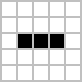
\includegraphics[height=.15\linewidth]{./images/blinker.png}
	\caption{Oscilador de periodo dos nombrado 'Blinker'}
\end{figure} 
\begin{figure}[H]
	
	\centering
	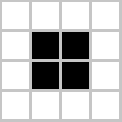
\includegraphics[height=.15\linewidth]{./images/block.png}
	\caption{Vida inmóvil nombrada 'Block'}
\end{figure} 

Debido al creciente interés, Conway propuso la búsqueda de una configuración inicial que podría crecer sin límite, la cual William Gosper encontró con la construcción de una configuración inicial de células que genera infinitos deslizadores durante su evolución. 

\begin{figure}[H]
	
	\centering
	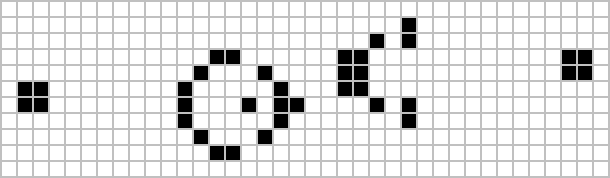
\includegraphics[scale=0.55]{./images/glider_gun.png}
	\caption{'Pistola de desplizadores' o 'Gosper glider gun' propuesta por William Gosper.}
	
\end{figure} 

Dada la popularidad del juego de vida, surge la necesidad de realizar simulaciones en los incipientes ordenadores y se enfrentan al problema de representar una malla infinita en un ordenador con memoria finita. Para ello se propone alterar las características topológicas de la malla, imitando las de una botella de Klein, una esfera, o un toro. En particular, esta última resulta atraer gran interés, pues se obtiene evidencia de que reduce los efectos asociados a la finitud de la malla \cite{finitudMalla, finitudMalla2}. Cabe descatar el estudio de la alteración de las cualidades geométricas de la malla, tales como el uso de figuras geométricas regulares diferentes al cuadrado (triángulo y hexágono)\cite{triangular}, teselaciones de Penrose \cite{penrose} o el empleo del espacio geométrico hiperbólico \cite{hiperbolico}. Finalmente, cabe notar que existen implementaciones en las cuales no se aplican condiciones sobre los bordes del dominio \cite{boardless}.

El juego de vida también muestra interesantes características en el campo de teoría de la computación. Pertenece a la clase IV de Wolfram \cite{ccuatro, ccuatro2} y se ha demostrado que es una máquina de Turing universal \cite{turingUniversal}. Por tanto existe una configuración inicial que simula una máquina de Turing, la cual fue extendida a una máquina universal de Turing \cite{turing}. Más recientemente en un esfuerzo colectivo, se ha implementado un ordenador con su propio lenguaje ensamblado, compilador a lenguaje de alto nivel, y sobre este último se ha implementado el conocido juego Tetris \cite{tetris, logical}.

En el juego de vida las células se actualizan simultáneamente en unidades de tiempo discretas, lo que implica que es un autómata celular síncrono. Si relajamos la condición de sincronicidad, obtenemos nuevos posibles esquemas de actualización, entre ellos el método guiado por pasos (step-driven), en el cual se decide la actualización de las células sin definir explicitamente el tiempo y el método guiado por tiempo (time-driven), en el cual cada célula tiene su propio reloj interno que marca su instante de actualización. Éste último ha sido estudiado en \cite{} sobre el juego de vida estocástico, esto es, cada célula tiene una probabilidad p de ser actualizada en cada unidad discreta de tiempo. Cuando $p=1$ obtenemos el juego de vida de Conway. Si 

En este trabajo emplearemos el método de Monte Carlo, a configuraciones en situación de $\alpha$-asincronicidad caracterizando su comportamiento a través de diferentes variables; el número de clusteres de células diferentes por unidad discreta de tiempo, su velocidad y densidad, entre otras, las cuales hasta donde podemos saber no han sido de interés en anteriores publicaciones. De esta manera podremos cuantificar el efecto de la $\alpha$-asincronicidad en configuraciones iniciales bien conocidas, tales como las comentadas anteriormente.

\end{document}

% !TeX root = ../proyecto.tex
